\documentclass[10pt]{beamer}

% --- Verzicht auf Themes für den "rohen" Look ---
% \usetheme{Madrid} <- Weglassen oder auskommentieren

% --- Schriften & Sprache ---
\usepackage[utf8]{inputenc}
\usepackage[ngerman]{babel}
\usepackage[T1]{fontenc}
\usepackage{lmodern} % Die klassische LaTeX-Schrift
\usepackage{caption}
\usepackage{listings}
\usepackage{xcolor}

% Definition der Farben
\definecolor{codegreen}{rgb}{0,0.6,0}
\definecolor{codegray}{rgb}{0.5,0.5,0.5}
\definecolor{codepurple}{rgb}{0.58,0,0.82}
\definecolor{backcolour}{rgb}{0.95,0.95,0.92}

% Allgemeine Styles für alle Codes
\lstset{
    backgroundcolor=\color{backcolour},   
    commentstyle=\color{codegreen},
    keywordstyle=\color{magenta},
    numberstyle=\tiny\color{codegray},
    stringstyle=\color{codepurple},
    basicstyle=\ttfamily\footnotesize, % Monospaced Schrift
    breakatwhitespace=false,         
    breaklines=true,                 
    captionpos=b,                    
    keepspaces=true,                 
    numbers=left,                    % Zeilennummern links
    numbersep=5pt,                  
    showspaces=false,                
    showstringspaces=false,
    showtabs=false,                  
    tabsize=2
}


% --- Metadaten ---
\title{PICasso}
\subtitle{PIC Microcontroller Simulator}
\author{Nik Wachsmann \& Ben Stahl}
\date{07.05.2026}

\begin{document}

\begin{frame}
    \titlepage
\end{frame}

\section{Einführung}

% --- Eine Folie ---
\begin{frame}{Einführung}
    \begin{columns}
        % Linke Spalte für Text
        \begin{column}{0.6\textwidth}
            \begin{itemize}
                \item Kein Schnickschnack.
                \item Nur Text und Struktur.
                \item Die mathematische Eleganz steht im Vordergrund:
            \end{itemize}
        \end{column}

        % Rechte Spalte für das Bild
        \begin{column}{0.4\textwidth}
            \centering
            % Ersetze 'beispielbild' durch deinen Dateinamen (ohne Endung)
            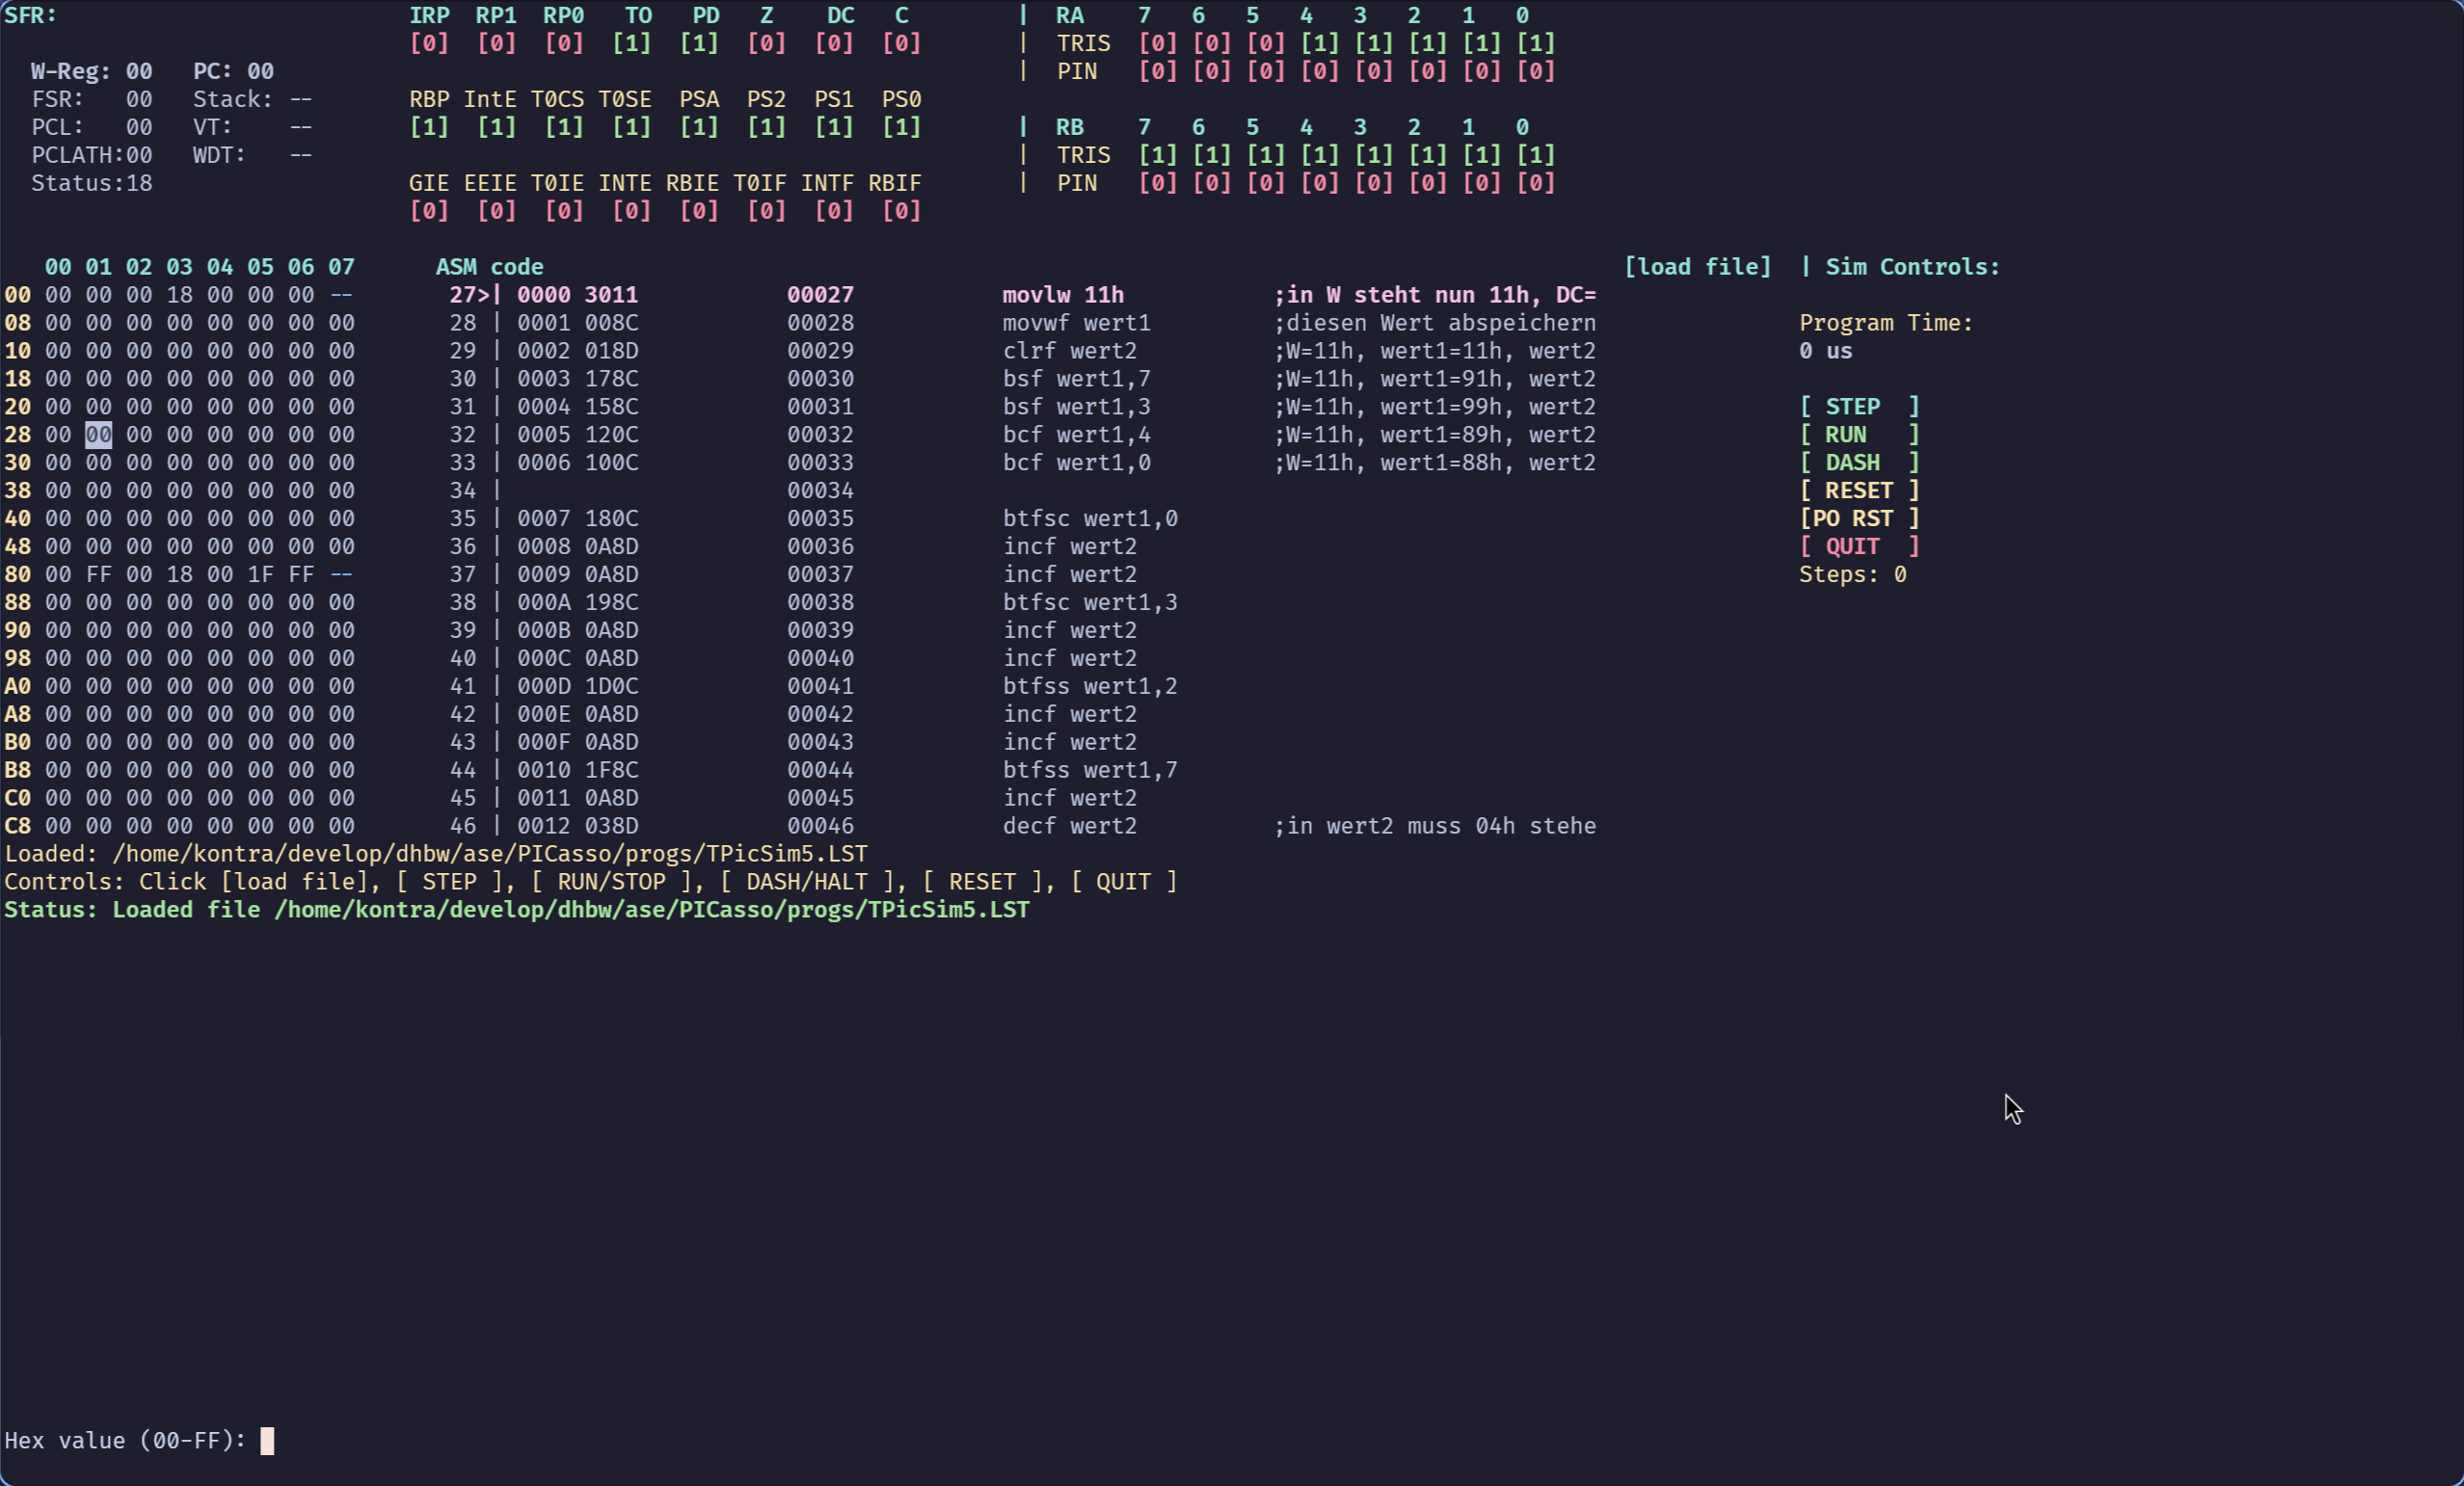
\includegraphics[width=\textwidth]{./images/pic2.png}
            \captionof{figure}{Bildunterschrift} % Optional
        \end{column}
    \end{columns}
\end{frame}
% --- Ende Folie ---

\begin{frame}[fragile]{Starten der Applikation}
    \begin{columns}
        \begin{column}{0.5\textwidth}
                \begin{enumerate}
        \item C++17-kompatibler Compiler (z.B. g++ $\ge$ 9)
        \item CMake $\ge$ 3.14
        \item ncurses-Bibliothek (libncurses-dev unter Linux)
    \end{enumerate}
        \end{column}
        \begin{column}{0.5\textwidth}
            \begin{lstlisting}[language=bash, caption=starten der Applikation]
git clone https://github.com/DefinitlyNotABot/PICasso.git
cd PICasso

make run
\end{lstlisting}
        \end{column}
    \end{columns}

\end{frame}

\begin{frame}{Aufzählungen}
    \begin{enumerate}
        \item Punkt Eins
        \item Punkt Zwei
    \end{enumerate}
\end{frame}

\end{document}